\documentclass[11pt,a4paper,oneside]{article}

%------------------
% Fonts and typsetting
\usepackage{color}
\usepackage[T1]{fontenc}        % 8-bit font encoding (256 glyphs)
\usepackage{amsfonts}		% additional characters in math mode
\usepackage{amsmath} 		%to use \text{}
\usepackage{amsfonts}		% additional characters in math mode
\usepackage{amsmath} 		%to use \text{ in math mode
\usepackage{fixltx2e}		%adds \textsubscript functionality

%------------------
% Page Layout
\usepackage[hmarginratio=1:1,top=32mm,columnsep=20pt]{geometry}
\usepackage{paralist}		% create compact itemize and enumerate lists (inparaenum and compactitem environments)

%------------------
% Floats 
\usepackage{graphicx}		%enables insertion of images
\newenvironment{Figure}		%floats are not allowed in multicols
	{\par\medskip\noindent\minipage{\linewidth}}
	{\endminipage\par\medskip}

\usepackage{float} 		%enables \figure[H] or [h!]
\usepackage{booktabs}		%for professional looking tables
\usepackage{multicol}		% enable multicolumn formatting of tables
\usepackage{caption}
\captionsetup{font=small,labelfont=bf}
\usepackage{capt-of}		%for captions in multicol environment
\usepackage{calc}		% arithmetic operations, useful for 4*\textwidth..etc
\usepackage{tikz}
\usetikzlibrary{shapes.geometric, arrows}

%------------------
% Code
\usepackage{algorithm}
\usepackage{algorithmicx}
\usepackage{algpseudocode}

%------------------
% Hyperref
\usepackage{hyperref}
\hypersetup{pdftex,
linktocpage=true,
bookmarks=true,
colorlinks=true,
citecolor=black,
filecolor=black,
linkcolor=black,
urlcolor=black}
\usepackage[all]{hypcap}	% points hyperlinks to the top of the image instead of caption text

%------------------
% Header / Footer
\usepackage{fancyhdr}
\pagestyle{fancy}
\lhead{}
\chead{}
\rhead{{October 2013}}
\lfoot{}
\cfoot{\thepage}
\rfoot{}

%------------------
% Abstract
\usepackage{abstract}

%------------------
% Lettrines
\usepackage{lettrine}

%------------------
% Metadata
\title{\vspace{-15mm}%
	\Large \textbf{Utilisation of Computer Algorithms in the Optimisation of Building Envelopes Thermal Performance}}
%\author{%
%	\textsc{Ayman Elmasry, Dr. Ahmed Atef and Dr. Hazem Eldaly}\\
%	\normalsize Dpt. of Architecture, Engineering Faculty, Ain Shams University
%	}
\date{}	

\begin{document}
\maketitle
\vspace{-1.5cm}
\begin{abstract}
\noindent As the architect is exposed to modern tools of architectural design such as computer simulation and architectural form generation, the architect is also exposed to technical difficulties which arise with them due to the fact that those tools require knowledge of computer programming, mathematics and physics that is not part of the standard architectural curriculum. This article introduces the architect to the process of thermal design by simulation and optimisation of building envelopes using computer algorithms and environmental simulation programmes, and in the process explain the essential concepts of computer programming and how it is integrated into the architectural design process to achieve thermally efficient designs.

\noindent The reader is introduced to computer programming from a theoretical point of view, with an explanation of the type of input needed by the computer algorithms in order to function properly, the different types of algorithms and their output, how to define the optimisation problem and its variables, and the different types of 3D virtual modelling and environmental simulation programmes and their role in the process.

\noindent Ultimately, the process is broken down into: \begin{inparaenum} \item building envelope analysis in terms of geometry and thermal variables, \item selection of suitable modelling and simulation programmes, \item choosing the most suitable algorithm, and finally \item the integration of the previous steps into a complete process with practical usable results.\end{inparaenum}
\end{abstract}

\begin{multicols}{2}

\section*{Introduction}

Thermal comfort and internal temperatures of a building space are primarily a function of building envelope design, the building element which controls the inward and outward flow of energy and matter, and architects have been faced with the dilemma of balancing the aesthetic element of envelopes with its thermal properties and performance --- among other things --- for as long as the profession has existed.

The methods used to handle this dilemma have been numerous and vary by different conditions such as climate, available materials and resources, available building technologies\ldots{}etc. Theories have been formulated to assist the architect in his endeavour to control the thermal performance of buildings; however, the results are never full-proof and will always vary due to the large number of variables and constraints that are part of the thermal equation.

With the development of modern science and the emergence of the computer age, new tools have been introduced to the process of architectural design to assist in the thermal design of building and in particular building envelopes, the latest of which is the the use of computer algorithms in the automated generation of building envelopes through the environmental simulation of virtual building models and feeding the results to a programme that evaluates the results and searches for the best solutions, adjusting the variables accordingly.

However, as the architect approaches this method, he is faced with technical difficulties which require knowledge of computer programming, mathematical optimisation and physics. Therefore, an introduction to the process of algorithmic design of building envelopes is needed, and is the purpose of this article.

\section{Algorithms and How they Function}

Algorithms are descriptions of steps to accomplish a specific task which allow the abstraction of a problem into parameters, or variables, and procedures, which are the detailed instructions given to the computer. The user inputs values of parameters, and the computer then calculates the outputs according the given procedure. The problem at hand is how to use these algorithms to create a computer programme that would analyse the building form and feed back the optimum solutions to the user (\emph{i.e.} the architect). 

	\paragraph{Building Geometry as Variables}\mbox{}\\[3mm]
The first step towards achieving this goal is understand the input needed by the algorithm (the algorithm being basically computer code); the building envelope has to analysed and broken down into variables and values. As any architect knows; geometry is built up from a point, to a line, to plane and to a solid. If the user of the algorithm can translate building geometry into at least the basic building block of any geometry, then the entry of building envelope data in a form that the algorithm can understand is possible.

The minimum requirement is to create a procedure for creating a point in space; this procedure will be defined for the algorithm as follows:
\begin{compactitem}[\footnotesize$\bullet$]
\item	{Procedure Handle\footnote{Handle: Name}:} Point\_A
\item	{Parameters/Variables:} Cartesian Coordinates $(x,y,z)$
\item	{Values:} $(0,0,0)$
\end{compactitem}
Then, the point procedure would be embedded --- or nested --- within a line procedure twice with different values for each procedure:
\begin{compactitem}[\footnotesize$\bullet$]
\item	{Procedure Handle:} Line\_A
\item	{Parameters/Variables:} ({Point\_A , Point\_B})
\item	{Values:} $[(x,y,z),(u,v,w)]$
\end{compactitem}
The process is repeated in the same manner until a solid geometry is formed (Fig. \ref{fig:Box}).

\begin{Figure}
	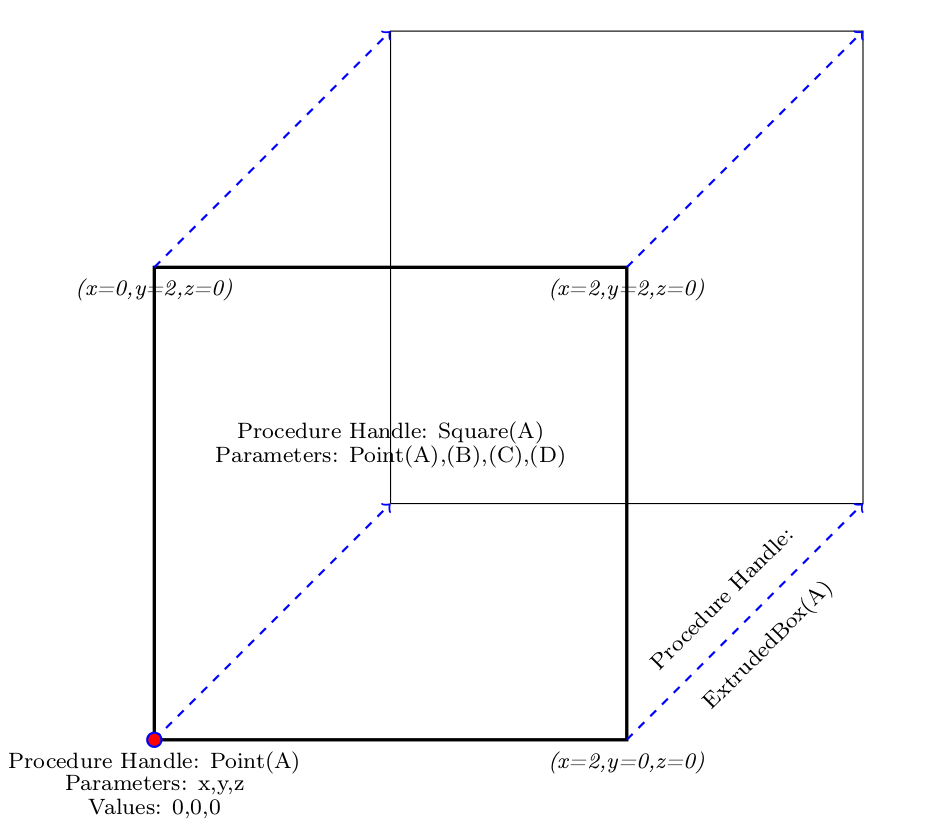
\includegraphics[width=\linewidth]{./Images/1-Box}
	\captionof{figure}{Procedures used to define a cuboid form}
	\label{fig:Box}
\end{Figure}

\section{Algorithmic Architecture}

Now that the general description and functionality of computer algorithms has been provided, a closer look at the different types of algorithms and their purposes is naturally the next step.

As far as architectural design is concerned; algorithms can be divided into two main types: \emph{Generative} and \emph{Performative}. \cite{fasoulaki08}

	\paragraph{Generative Algorithms}\mbox{}\\[3mm]
Architectural generative design is a process which uses \emph{rule-based}\footnote{\emph{Rule-based}: consisting of a solid set of consecutive instructions that govern an action to produce a desired outcome} algorithms, governed by repetitive patterns and shape transformations; these algorithms can be fully automated or user controlled in a step-by-step manner. What differentiates generative algorithms from each other are the form generating systems which drive the algorithm, usually adopted from naturally occurring behaviour of living organisms. \cite{arida04}

Prominent generative algorithms used for architectural form generation purposes include:
\begin{compactenum}[\indent 1.]
\item Cellular Automata;
\item Voronoi Diagrams;
\item Fractals;
\item Shape Grammars; and
\item L-System.
\end{compactenum}

Out of the above, two examples are explained briefly here. Cellular Automata is a computational method which can simulate complex growth systems using simple rules, the initial configuration would include at least one cell (Fig. \ref{fig:CellularAuto}).

\begin{Figure}
	\centering	
	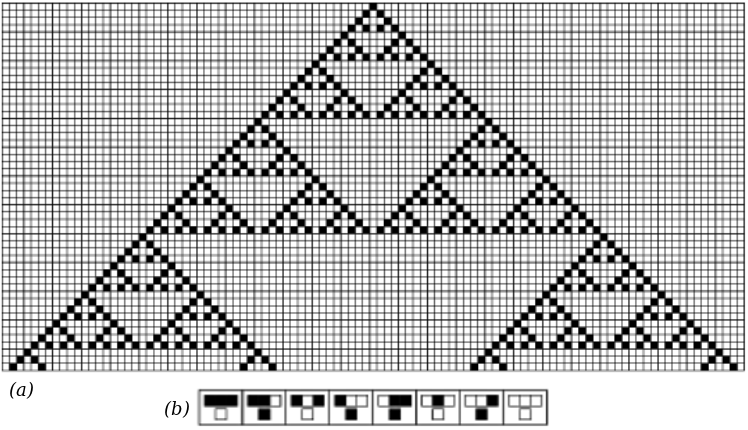
\includegraphics[width=\linewidth]{./Images/2-CellularAutomata}
	\captionof{figure}{An example of cellular automata showing (a) the sequence of generations and (b) the governing rule. \cite{wolfram02}}
	\label{fig:CellularAuto}
\end{Figure}

A Voronoi Diagram is a way of decomposing a space into regions, which is a process initiated with a set of points in space called generating points; then, lines are drawn from an equal distance from each two points, creating polygons or cells (Fig \ref{fig:Voronoi}).

\begin{Figure}
	\centering
	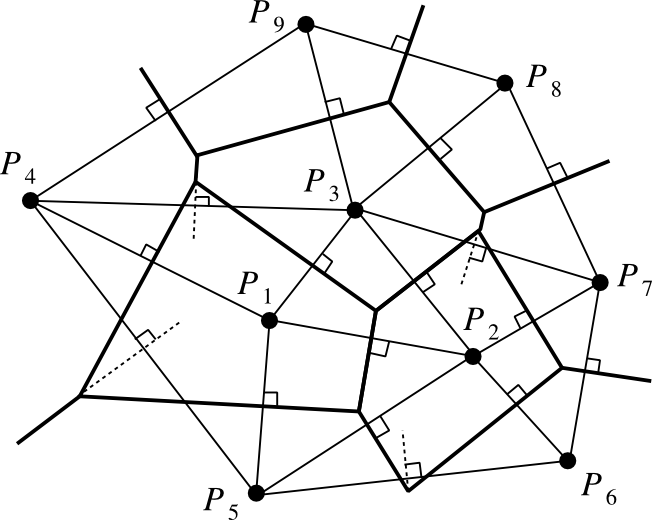
\includegraphics[width=0.8\linewidth]{./Images/3-VoronoiDiagram}
	\captionof{figure}{A Voronoi Diagram \cite{fujita00}}
	\label{fig:Voronoi}
\end{Figure}

	\paragraph{Performative Algorithms}\mbox{}\\

	These types of algorithms are based on what is called optimisation algorithms; which would take a certain aspect of the building performance --- thermal performance of the envelope in this particular case --- and searches for solutions that would enhance the performance, ultimately finding the best solution. The underlying process of Performative Algorithms is called \emph{Mathematical Optimisation}.

		\subparagraph{Mathematical Optimisation}

		Optimisation mathematics and programming is called a \emph{search method}, which searches for and locates the \emph{optimum} solution. The optimum solution can be the maxium value of a function, or the minimum value of a function; therefore, all mathematical optimisation operations are either called \emph{minimisation} or \emph{maximisation} problems.

		The general mathematical form of unconstrained optimisation is:\\
\begin{equation}
\text{min} f(x), x=[x_1,x_2\dots,x_n]^T \in \mathbb{R}
\end{equation}
The continuous components of $x$ are called the design variables, and $f(x)$ is the objective function. The optimum vector that solves the equation is denoted by \textbf{x*} with a corresponding optimum function value of $f(\text{\textbf{x*}})$ (Fig. \ref{fig:LocalOptimum}).

		The full process of mathematical optimisation is to take a real world problem (\emph{e.g.} thermal performance of a building envelope), construct it into a mathematical model of fixed parameters and variables, then process it through the optimisation algorithm, leading to the practical implication of the optimum solution (Fig. \ref{fig:OptimisationModel}).

\end{multicols}
\begin{Figure}
	\centering
	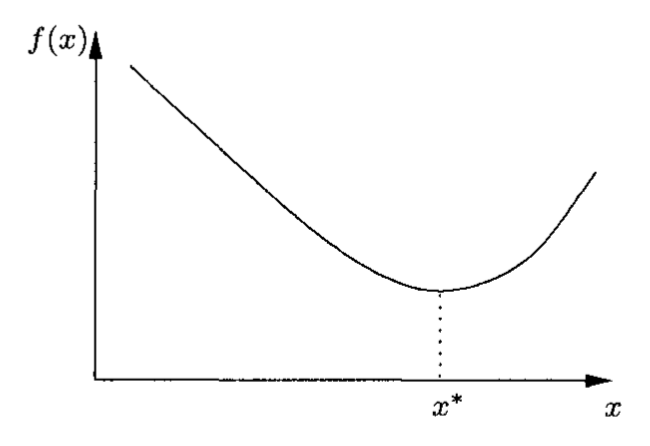
\includegraphics[width=0.6\linewidth]{./Images/4-LocalOptimum}
	\captionof{figure}{A single variable function with the optimum at \textbf{x*} \cite{snyman05}}
	\label{fig:LocalOptimum}
\end{Figure}

\begin{Figure}
	\centering	
	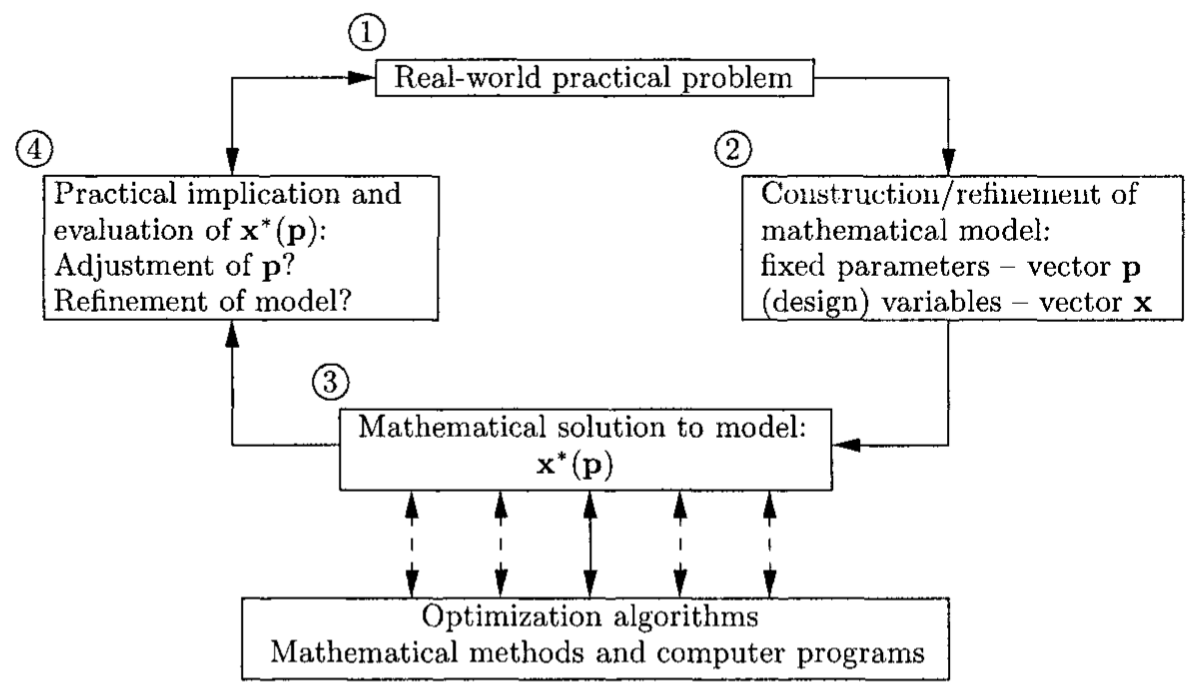
\includegraphics[width=0.7\linewidth]{./Images/5-OptimisationModel}
	\captionof{figure}{The Mathematical Optimisation Modelling Process \cite{snyman05}}
	\label{fig:OptimisationModel}
\end{Figure}
\begin{multicols}{2}

	\paragraph{Types of Optimisation Algorithms}
	Mathematical optimisation algorithms are numerous and differ greatly in solution space searching methods. The predominantly common algorithms in architectural applications are:
	\begin{compactenum}
	\item Genetic Algorithm
	\item Simmulated Annaeling
	\item Tabu Search
	\end{compactenum}
	It should be noted that although the three are very different in terms of origin and search method, they have one thing in common which is being under the \emph{Metaheuristic}\footnote{\emph{Metaheuristic}: an algorithm which guides a heuristic (self learning) search method} class of mathematical optimisation algorithms.
	
	\subparagraph{Genetic Algorithm}

	Genetic Algorithms are \emph{evolutionary} algorithms which simulate biological evolution, and draws most of its terminology from biological evolutionary science.

	The process of optimisation using GA can be described as follows: ``Under GA terminology, a solution to a problem is an \emph{individual}, and the group of solutions existent at each stage is a \emph{population}. Each time a new population of individuals is created it is called a \emph{generation}. In binary GA's[\dots]each individual is represented by a binary string called \emph{chromosome}, which encodes all parameters of interest corresponding to that individual. A chromosome of formed of \emph{alleles}; the binary coding bits. The fitness of any particular individual corresponds to the value of the objective function at that point''. \cite{caldas01}

	An \emph{initial population} is randomly generated, with each of the individuals coded with different \emph{genetic} design variables (using the notion of chromosomes), then a number of stochastic operators start to manipulate the initial population, including \begin{inparaenum} \item \emph{crossovers}; the swapping of parts of chromosome values between different individuals, and \item \emph{mutation}; introducing new values randomly to some individuals to create diversity.\end{inparaenum}

	Finally an elitist model is created from the best set of solutions in this generation, and is used as the initial population of the next generation, and the same loop keeps repeating until the termination criteria of the GA are met and the final set of solutions are recorded (see Fig. \ref{fig:GA}).

	\begin{Figure}
		\centering
		\includegraphics[height=7cm]{./Images/6-GA}
		\captionof{figure}{Flowchart showing stages of GA}
		\label{fig:GA}
	\end{Figure}

	\subparagraph{Simmulated Annaeling}

	Simmulated Annaeling is as mathematical optimisation method. It draws its terminology from the metallurgical process of annealing which is the heating and controlled cooling of metals to reach its ground state with the lowest internal energy \cite{lam88}. This search method is also Metaheuristic, with emphasis on find the \emph{global} maximum or minimum. The process of Simmulated Annealing is described by the following algorithm (in pseudocode):\\
	
		\begin{algorithmic}[1]
			\State Get an initial state with energy $x$
			\State Make the initial state the current state
			\State Select an initial high temperature $T$
			\While {System is not yet frozen}
			\While {System is not yet in thermal equilibrium}
				\State pick a random nearby state with energy $x_p$
				\State let $\Delta x = x_p - x$
				\If {$\Delta x \leq 0$}
					\State the new state becomes the current state
				\Else
					\State reject state
				\EndIf
			\EndWhile
			\State Reduce the temperature $T$ by $\Delta T$
			\EndWhile
			\State Output the current state
		\end{algorithmic}

	\subparagraph{Tabu Search}

	Tabu Search depends on what are called \emph{adaptive memory} and {responsive expolration}. The basic principle is that it heavely uses different memory-based techniques to \begin{inparaenum} \item avoid revisiting previously tested solutions, \item to memorise elements that are common among good solutions, and \item the impact of choices made till a certain point on the progress of the search to find the optimum solution, which is an added level of self-learning.\end{inparaenum}

	This makes Tabu Search a very intelligent search method, which is very efficient at find the optimum solutions in large solution spaces, or to complex problems.

\section{Thermal Aspect of the Optimisational Problem}

Having explained the mathematical and basic programming concepts behind optimisation algorithms, the next step is to define the function in question; the \emph{objective function}. In this particular case the objective function is the thermal performance of building envelopes. The exchange of heat between the building and external environment is expressed in the following equation:
\begin{equation}
	Qi\pm Qc\pm Qs\pm Qv-Qe=\Delta S
\end{equation}
\footnotesize
\indent$Qi=$Internal heat gain\\
\indent$Qc=$Conduction heat gain or loss\\
\indent$Qs=$Solar heat gain\\
\indent$Qv=$Ventilation heat gain or loss\\
\indent$Qe=$Evaporation heat loss\\
\indent$\Delta S=$Difference in stored heat\\
\normalsize

Given that solar radiation is the most significant variable in the above equation \cite{szokolay08}, it would be benefitial --- for the sake of simplicity --- to focus on the aspect of passive solar design when considering the thermal performance of building envelopes.

\paragraph{Passive Solar Control Design Variables}\mbox{}\\

The previously mentioned function variables in optimisation problem of building envelope thermal performance through passive solar control can be any of the architectural elements shown in following table:

\begin{table}[H]
	\centering
	\begin{tabular}{l|l}
		\textbf{Shape}&Surface-to-Volume Ratio\\
		&Orientation\\
		&\\
		\textbf{Fabric}&Shading\\
		&Surface Material Properties\\
		&\\
		\textbf{Fenestration}&Size, Position and Orientation\\
		&Glazing Material\\
		&Closing Mechanism\\
		&External Shading\\
	\end{tabular}
	\caption{Passive Thermal Control Design Variables}
	\label{tab:ThermalDesignVariables}
\end{table}

Now that the thermal variables which would enable us to control the thermal performance are defined, and the theoritcal method of modelling them into a mathematical function illustrated; a practical way of measuring and optimising the thermal performance of the building envelope is the next step. 

\paragraph{Building Modelling and Simulation}\mbox{}\\

There several methods for modelling and simulation (energy simulation) of building elements; the one discussed herein, and the most practical, is the use of Environmental/Energy Modelling and Simulatin computer programmes. There are two main advantage of these programmes:
\begin{compactenum}
	\item They save the user the hassle of modelling the physical properties and reactions of building elements into equations, which are pre-programmed in the simulation application, and measures the impact of different variables with different values on the overall thermal performance.
	\item The variable values can later on be manipulated by the optimisation algorithm to search for the optimum values through repeated simmulation of different values, thus reaching the optimum solution for each variable, or for overall optimum performance in multi-variable cases.
\end{compactenum}




\end{multicols}

\bibliographystyle{unsrt}
\bibliography{./Bibliography}

\end{document}
